\documentclass[UTF8,a4paper,12pt]{ctexart}
\usepackage[margin=2.5cm]{geometry}
\usepackage{amsmath,amssymb}
\usepackage{graphicx}
\usepackage{booktabs}
\usepackage{tabularx}
\usepackage{array}
\usepackage{float}
\usepackage{hyperref}
\usepackage{xcolor}
\usepackage{listings}
\usepackage{caption}
\usepackage{tikz}
\usetikzlibrary{arrows.meta,positioning,fit,backgrounds}
\hypersetup{colorlinks=true,linkcolor=blue,urlcolor=blue,citecolor=blue}
\graphicspath{{./}}
\lstset{
  basicstyle=\ttfamily\small,
  breaklines=true,
  columns=fullflexible,
  frame=single,
  backgroundcolor=\color{gray!6}
}

\title{基于 GAN 的 CIFAR-10 图像生成实验报告}
\author{
谢其虎\thanks{共同第一作者。}
\and
蒋世航\footnotemark[1]
\and
陈乐韬\footnotemark[1]
}
\date{}

\begin{document}
\maketitle


\section{摘要}

生成对抗网络（Generative Adversarial Networks, GANs）通过生成器与判别器之间的极小极大博弈学习真实数据分布，是图像生成任务中的经典方法。本文围绕 CIFAR-10 图像生成任务，系统实现并比较了多种 GAN 训练策略，包括 DCGAN、WGAN-GP、类条件 GAN、ResNet 条件 GAN、DiffAugment、最小二乘 GAN 损失以及指数滑动平均（Exponential Moving Average, EMA）生成器。实验在本地 CIFAR-10 数据集上完成，使用 5000 个生成样本通过预训练 Inception 网络计算 Fréchet Inception Distance（FID）和 Inception Score（IS）。实验结果表明，在当前实现与训练预算下，简单但容量更大的 DCGAN 配合 BCE 对抗损失取得最佳结果：160 通道 DCGAN 的 raw generator 将 FID 降至 \textbf{31.678}，IS 提升至 \textbf{5.872 ± 0.161}。相较于 50 epoch DCGAN 基线，FID 从 38.290 降低约 17.3\%，IS 从 5.346 提升约 9.9\%。该结果说明，对于 CIFAR-10 这类低分辨率数据集，稳定训练、适当扩展模型容量和参数平均策略往往比直接堆叠更复杂结构更可靠。


\section{引言}

CIFAR-10 是图像生成任务中常用的低分辨率自然图像数据集，包含 airplane、automobile、bird、cat、deer、dog、frog、horse、ship 和 truck 共 10 个类别。尽管 CIFAR-10 图像尺寸仅为 32×32，其类别多样性、细粒度结构和复杂背景仍然使生成任务具有挑战性：模型不仅需要生成自然的颜色和纹理，还需要保持可辨识的目标形状与类别语义。


近年来，生成式模型在计算机视觉中得到广泛应用，典型任务包括无条件图像生成、类别可控图像生成、图像修复、风格迁移和数据增强等。与传统判别式模型不同，生成模型需要直接刻画数据分布本身，因此不仅要关注单张图像是否清晰，还要关注整体样本集合是否具有足够的多样性，以及生成分布是否覆盖真实数据中的主要语义模式。对于 CIFAR-10 这样的课程实验数据集而言，图像尺寸较小、训练成本相对可控，适合在有限计算资源下比较不同 GAN 结构和训练策略。


GAN 的核心思想是同时训练两个神经网络：生成器从随机噪声中合成图像，判别器区分真实图像与生成图像。理想情况下，生成器逐渐逼近真实数据分布，判别器无法可靠地区分真假样本。然而在实际训练中，GAN 常出现梯度不稳定、模式坍塌、样本模糊、类别混淆等问题。因此，本项目不仅实现基础 GAN，还进一步探索多种常见改进策略，目标是在可运行、可复现的代码框架下尽可能提升 CIFAR-10 生成质量。


本项目选择 GAN 图像生成方向而非对抗防御方向，主要原因在于图像生成结果具有较强的可视化解释性，能够通过样本图、训练过程图和定量指标共同分析模型行为。同时，GAN 训练过程对网络结构、损失函数、优化器超参数和正则化策略都较为敏感，适合作为理解深度生成模型训练机制的综合实验。为了避免只停留在单一模型复现层面，本文从基础 DCGAN 出发，逐步加入 WGAN-GP、类别条件、投影判别器、ResNet 结构、DiffAugment、LSGAN 损失和 EMA 生成器等策略，并在统一评价流程下比较其效果。


本文关注的核心问题包括：第一，基础 DCGAN 在 CIFAR-10 上能够达到怎样的生成质量；第二，WGAN-GP、条件建模和数据增强等改进是否能在相同训练预算下带来稳定提升；第三，FID、IS 与可视化样本之间是否给出一致的模型优劣判断。围绕这些问题，实验不仅报告最终最优模型，也分析了若干复杂方法未能超过简单基线的原因。


本文的主要贡献如下：


\begin{enumerate}
\item 实现了完整的 CIFAR-10 GAN 训练、采样和评估流水线，支持本地数据读取，无需重复下载数据集。
\item 比较了 DCGAN、WGAN-GP、条件 GAN、ResNet 条件 GAN、DiffAugment、LSGAN 和 EMA 等多种结构与训练策略。
\item 使用 FID 和 IS 对所有主要模型进行统一评估，并给出可视化样本图和类别级展示图。
\item 通过实验发现，在当前训练设置下，\textbf{160 通道 DCGAN + BCE 损失}取得最佳结果，其中 raw generator 同时获得最低 FID 和最高 IS。
\end{enumerate}


\section{相关工作}

\subsection{生成对抗网络}

GAN（Generative Adversarial Network，生成对抗网络）最早由 Ian Goodfellow 等人在 2014 年提出，是一种基于对抗学习（Adversarial Learning）的深度生成模型，其核心目标是通过学习真实数据分布来生成与真实样本高度相似的数据。GAN由生成器（Generator）和判别器（Discriminator）两部分组成：生成器以随机噪声为输入，学习将低维潜在空间映射到数据空间，从而生成逼真的样本；判别器则负责区分输入样本来自真实数据分布还是由生成器产生的伪造样本。二者通过极小极大（Min-Max）博弈的方式进行联合优化，即生成器不断提升“以假乱真”的能力，而判别器不断增强辨别真伪的能力。在理想情况下，当生成分布逐渐逼近真实数据分布时，判别器将无法区分真实样本和生成样本。原始GAN采用基于二元交叉熵（Binary Cross-Entropy, BCE）的对抗目标函数，但由于其目标函数对应的 Jensen–Shannon divergence 散度在真实分布与生成分布支撑集重叠较小时容易饱和，因此训练过程中经常出现梯度消失、模式崩溃（Mode Collapse）以及训练不稳定等问题。尽管存在上述局限性，GAN所提出的对抗学习范式极大推动了生成模型的发展，并在图像生成、图像编辑、超分辨率重建、图像到图像翻译以及无监督表示学习等领域取得了广泛成功，成为现代生成式人工智能的重要基础之一。


原始 GAN 的理论目标可以写为如下极小极大优化问题：


$$
\min_G \max_D V(D,G)
= \mathbb{E}_{x \sim p_{data}(x)}[\log D(x)]
+ \mathbb{E}_{z \sim p_z(z)}[\log(1-D(G(z)))].
$$


其中，$p_{data}$ 表示真实数据分布，$p_z$ 表示潜在噪声分布，$G(z)$ 表示由生成器产生的伪样本，$D(x)$ 表示判别器判断输入样本为真实样本的概率。判别器希望最大化该目标，即提高真实样本得分并降低生成样本得分；生成器则希望最小化该目标，使 $D(G(z))$ 尽可能接近真实样本。实际训练时通常交替更新 $D$ 和 $G$，并常采用非饱和生成器损失以缓解早期训练中的梯度不足问题。


\begin{figure}[H]
\centering
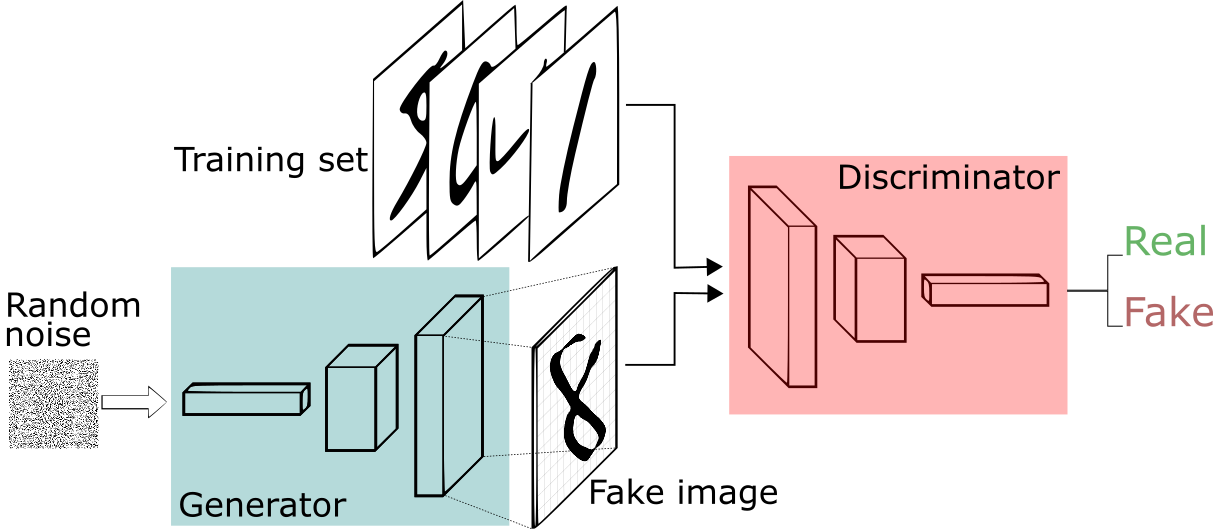
\includegraphics[width=0.75\linewidth]{figures/GAN.png}
\caption{GAN}
\end{figure}


\subsection{DCGAN}

DCGAN 将卷积神经网络引入 GAN 框架，使用转置卷积构建生成器，并使用卷积下采样构建判别器。相比全连接 GAN，DCGAN 更适合图像数据，能够学习局部纹理和空间结构。DCGAN 还引入了 Batch Normalization、ReLU、LeakyReLU 等实践经验，成为许多图像生成实验的基础架构。本文将 DCGAN 作为主要基线，并进一步调整模型容量和训练长度。


在 CIFAR-10 这类小尺寸图像上，DCGAN 的优势在于结构清晰、训练速度较快，并且能够较直接地观察损失函数和模型容量变化对生成结果的影响。本文使用 DCGAN 作为所有改进策略的参照系：一方面通过 50 epoch 基线评估基本生成能力，另一方面通过延长训练、增加通道数和引入 EMA 观察简单模型在充分优化后的上限。


\subsection{WGAN-GP}

WGAN 使用 Wasserstein 距离替代 Jensen-Shannon 散度以改善训练稳定性。WGAN-GP 进一步用梯度惩罚约束判别器满足 Lipschitz 条件，通常可以缓解训练震荡和梯度消失问题。但 WGAN-GP 需要更多判别器更新步数，训练成本更高，且在小模型和有限训练预算下未必一定提升最终 FID。本文将 WGAN-GP 作为重要对比方法。


与普通 GAN 中输出真假概率的判别器不同，WGAN-GP 中的判别器通常被称为 critic，其输出不经过 Sigmoid，而是作为 Wasserstein 距离估计的一部分。该方法更关注真实分布与生成分布之间的连续距离，因此在许多任务中训练曲线更具可解释性。本文将其纳入对比，是为了检验更稳定的理论目标在本项目有限 epoch 与固定网络容量下是否能转化为更好的 FID 和 IS。


\subsection{条件 GAN 与投影判别器}

条件 GAN 将类别标签作为额外输入，使生成器能够按指定类别生成图像。相比无条件 GAN，条件 GAN 能够提供更可控的生成结果，但同时也需要模型学习图像分布与类别条件之间的对应关系。本文实现了 CNN 条件 GAN，并进一步尝试 ResNet 条件生成器与投影判别器，以增强类别条件建模能力。


对于 CIFAR-10，类别标签提供了非常直接的监督信号。条件 GAN 理论上可以减少生成分布的不确定性，使模型分别学习十个类别下的图像分布；但另一方面，判别器也需要同时判断图像真实性和标签一致性，这会提高优化难度。投影判别器通过图像特征与类别嵌入之间的内积建模标签条件，相比简单拼接标签更适合类别条件图像生成，因此本文在条件模型中采用该设计。


\subsection{DiffAugment 与 EMA}

DiffAugment 在判别器输入端对真实图像和生成图像施加可微数据增强，例如颜色扰动、平移和 cutout，以降低判别器过拟合风险。EMA 则维护生成器参数的指数滑动平均版本，常用于改善采样阶段的稳定性与视觉质量。本文分别测试了 DiffAugment 和 EMA 在不同 GAN 架构中的作用。


在数据量有限或判别器较强时，判别器可能快速记住训练图像的局部细节，导致生成器获得的梯度质量下降。DiffAugment 的特点是同时作用于真实样本和生成样本，并保持增强操作可微，因此不会切断生成器的反向传播路径。EMA 则不改变训练目标，而是在参数层面对生成器进行时间平均，通常可以获得更平滑的采样模型。二者分别从输入扰动和参数平滑两个角度改善训练过程，是本文方法比较中的重要辅助策略。


\section{方法}

\subsection{任务定义}

给定真实图像数据集 $\mathcal{D} = \{x_i\}_{i=1}^{N}$，其中 $x_i \in \mathbb{R}^{3 \times 32 \times 32}$，目标是学习一个生成器 $G_\theta$，使其能够将随机噪声 $z \sim \mathcal{N}(0, I)$ 映射为逼近真实 CIFAR-10 分布的图像：


$$
\hat{x} = G_\theta(z).
$$


判别器 $D_\phi$ 接收图像并输出真假判别分数。训练目标是使生成器生成的样本尽可能接近真实图像分布，同时使判别器无法区分真假图像。


在无条件生成设置中，$G_\theta$ 只接收随机噪声 $z$，模型需要直接学习 CIFAR-10 十个类别混合后的总体分布。在条件生成设置中，模型额外接收类别标签 $y \in \{0,\dots,9\}$，目标变为学习条件分布 $p(x|y)$，即在指定类别条件下生成对应语义的图像。本文同时实现无条件和有条件两类模型，但最终主要根据 FID 和 IS 选择无条件 DCGAN 作为最优结果。


所有训练图像首先经过随机水平翻转，然后通过 \texttt{ToTensor} 转换为张量，并按通道归一化到 $[-1,1]$。这一范围与生成器末端的 Tanh 激活函数一致，使真实图像和生成图像处于相同数值空间。采样和评价时，再将生成图像从 $[-1,1]$ 映射回 $[0,1]$，用于保存可视化图像和输入 Inception 网络计算指标。


\subsection{DCGAN 基线}

DCGAN 生成器由多层转置卷积组成。输入噪声维度为 128，先通过 $4\times4$ 转置卷积映射为高维空间特征，再经过三次上采样得到 $32\times32$ RGB 图像。每个中间层使用 Batch Normalization 和 ReLU，以稳定特征分布并提高非线性表达能力。生成器最后使用 Tanh 激活函数，将输出限制在 $[-1, 1]$。


判别器采用与生成器近似对称的卷积下采样结构。输入图像依次经过步长为 2 的卷积层压缩空间分辨率，并通过 LeakyReLU 提供负半轴梯度，最后输出一个标量真假分数。本文的基础通道数设置为 64，并进一步测试通道数为 96 的更大模型。权重初始化采用 DCGAN 常用的正态初始化：卷积层权重均值为 0、标准差为 0.02，BatchNorm 层权重均值为 1、标准差为 0.02，偏置初始化为 0。


基础 DCGAN 使用二元交叉熵损失：


$$
\mathcal{L}_D =
-\mathbb{E}_{x \sim p_{data}}[\log D(x)]
-\mathbb{E}_{z \sim p_z}[\log(1-D(G(z)))],
$$


$$
\mathcal{L}_G =
-\mathbb{E}_{z \sim p_z}[\log D(G(z))].
$$


在代码实现中，判别器输出未经过 Sigmoid，而是直接作为 logits 输入 \texttt{BCEWithLogitsLoss}，这样可以避免显式 Sigmoid 带来的数值不稳定。训练时先固定生成器更新判别器，使其提高真实图像和生成图像的区分能力；随后固定判别器更新生成器，使生成图像被判别器判断为真实。该交替优化过程在每个 mini-batch 上执行一次。


\subsection{WGAN-GP}

WGAN-GP 将判别器解释为 critic，优化 Wasserstein 距离近似。其判别器损失为：


$$
\mathcal{L}_D =
\mathbb{E}_{z \sim p_z}[D(G(z))]
-\mathbb{E}_{x \sim p_{data}}[D(x)]
+ \lambda \mathbb{E}_{\hat{x}}[(\|\nabla_{\hat{x}}D(\hat{x})\|_2 - 1)^2],
$$


其中 $\hat{x}$ 是真实样本与生成样本之间的线性插值，$\lambda$ 为梯度惩罚系数，实验中设为 10。生成器目标为最小化：


$$
\mathcal{L}_G = -\mathbb{E}_{z \sim p_z}[D(G(z))].
$$


本文的 WGAN-GP 与 DCGAN 使用相同的卷积生成器和判别器骨架，但训练目标和优化设置不同。critic 不输出概率，而是输出未归一化的实数评分；训练时每进行一次生成器更新前，critic 会进行多次更新，实验中设置 \texttt{n\_critic=5}。梯度惩罚项在真实图像和生成图像之间随机线性插值得到的样本 $\hat{x}$ 上计算，用于约束 critic 关于输入图像的梯度范数接近 1。由于 WGAN-GP 每个 batch 需要额外计算输入梯度，其单位 epoch 训练开销明显高于普通 DCGAN。


\subsection{条件 GAN}

条件 GAN 将类别标签 $y$ 输入生成器，使模型学习条件分布 $p(x|y)$：


$$
\hat{x} = G(z, y).
$$


CNN 条件生成器通过类别嵌入向量与噪声向量拼接实现条件控制。具体而言，标签 $y$ 先经过 Embedding 层得到低维类别向量，再与噪声 $z$ 在通道维度拼接，作为转置卷积生成器的输入。这样，生成器在合成图像时可以利用类别信息调整目标形状、纹理和背景分布。


判别器使用投影机制，将图像特征与类别嵌入相乘，从而判断图像是否既真实又符合对应类别。其输出可表示为：


$$
D(x,y)=h(f(x))+\langle v_y, f(x)\rangle,
$$


其中 $f(x)$ 是判别器提取的图像特征，$h(\cdot)$ 是无条件真假评分头，$v_y$ 是类别 $y$ 对应的嵌入向量。第一项判断图像整体真实性，第二项建模图像特征与类别标签之间的一致性。条件模型训练中使用 hinge loss：


$$
\mathcal{L}_D =
\mathbb{E}_{x,y}[\max(0,1-D(x,y))]
+\mathbb{E}_{z,y}[\max(0,1+D(G(z,y),y))],
$$


$$
\mathcal{L}_G =
-\mathbb{E}_{z,y}[D(G(z,y),y)].
$$


\subsection{ResNet 条件 GAN}

为了增强模型表达能力，本文进一步实现了基于残差块的条件生成器和判别器。ResNet 结构通过残差连接缓解深层网络训练难度，并理论上能够生成更复杂的纹理与结构。实验中使用 128 通道基础宽度，并结合 DiffAugment 与 EMA 训练。


ResNet 条件生成器首先将噪声向量通过全连接层投影为 $4\times4$ 的初始特征图，然后经过三个残差上采样块逐步恢复到 $32\times32$ 分辨率。每个生成器残差块使用条件 Batch Normalization，根据类别标签生成对应的缩放和偏移参数，使不同类别可以拥有不同的特征调制方式。判别器则由残差下采样块组成，并使用谱归一化约束卷积层和线性层权重，以增强判别器训练稳定性。最终判别器同样采用投影形式，将全局池化后的图像特征与类别嵌入结合得到条件真假评分。


与 CNN 条件 GAN 相比，ResNet 条件 GAN 的表达能力更强，但训练也更依赖超参数设置。学习率、BatchNorm 行为、判别器强度、DiffAugment 策略和 EMA decay 都会影响最终收敛状态。因此本文将其作为增强模型进行实验比较，而不是默认假设复杂结构一定优于 DCGAN 基线。


\subsection{DiffAugment}

DiffAugment 对真实图像和生成图像使用相同类型的可微增强，包括：


\begin{itemize}
\item color：颜色扰动；
\item translation：平移扰动；
\item cutout：随机遮挡。
\end{itemize}


该策略的目标是防止判别器过快记住训练集细节，从而为生成器提供更平滑、更有泛化性的梯度。


本文在训练判别器时，对真实图像和生成图像分别施加同一组增强策略；在训练生成器时，也对生成图像施加相同的可微增强后再输入判别器。这样可以保证生成器仍然能够通过增强操作获得有效梯度。具体实现中，color 包含亮度、饱和度和对比度扰动；translation 通过随机平移改变目标位置；cutout 在图像中随机遮挡一个局部区域。三种增强共同构成 \texttt{color,translation,cutout} 策略。


需要注意的是，DiffAugment 并不直接提升生成器容量，而是改变判别器看到的数据分布。如果增强强度或训练目标与当前模型不匹配，可能会使判别器学习到的边界变得过于平滑，从而影响生成器优化。因此本文将其作为消融因素，与 BCE、LSGAN、EMA 等策略共同比较。


\subsection{EMA Generator}

EMA 维护生成器参数的滑动平均：


$$
\theta_{EMA} \leftarrow \alpha \theta_{EMA} + (1-\alpha)\theta,
$$


其中 $\alpha=0.999$。训练过程中仍使用原始生成器进行反向传播，采样和评估时优先使用 EMA 生成器。EMA 通常可以减少单步参数震荡带来的采样质量波动。


本文在启用 EMA 时，会在每次生成器参数更新后同步更新一份 \texttt{ema\_model}。训练 checkpoint 中同时保存原始生成器和 EMA 生成器参数，因而后续可以分别评估 raw generator 与 EMA generator 的 FID/IS。这样的设计有助于判断 EMA 改进是否来自真实分布拟合能力提升，还是只是在采样阶段起到平滑作用。实验结果显示，EMA 在不同通道数和训练轮数下的收益并不完全一致：ch=160 的 raw generator 同时获得最低 FID 和最高 IS。


\subsection{训练与评估流程}

整体实验流程分为训练、采样、定量评估和可视化分析四个步骤。训练阶段读取本地 CIFAR-10 数据，按 mini-batch 交替更新判别器和生成器，并在每个 epoch 记录平均判别器损失、生成器损失和耗时。采样阶段固定一组随机噪声，定期保存生成图像网格，以观察模型从噪声纹理到语义结构逐渐形成的过程。checkpoint 按固定间隔保存，便于回溯不同训练轮数下的模型表现。


图~\ref{fig:method-pipeline} 展示了本文最终方法的训练与评估框架。训练阶段由两条输入流组成：一条是真实 CIFAR-10 mini-batch，另一条是从标准正态分布采样的潜在噪声。噪声经由 ch=160 的 DCGAN 生成器得到伪样本，真实样本和伪样本共同输入判别器，并通过 BCE 对抗损失交替更新生成器和判别器。训练过程中同时维护 EMA 生成器，并在 checkpoint 中保存 raw generator 与 EMA generator，以便后续分别评估二者的 FID/IS。


\begin{figure}[H]
\centering
\includegraphics[width=\linewidth]{figures/overview.png}
\caption{本文最终 DCGAN 方法的训练与评估流程。生成器和判别器通过 BCE 对抗损失交替优化；训练时同步维护 EMA 生成器；评估阶段分别加载 raw generator 和 EMA generator 计算 FID/IS，并生成样本图用于定性分析。}
\label{fig:method-pipeline}
\end{figure}



评估阶段使用独立脚本从指定 checkpoint 中加载生成器，采样 5000 张图像，并使用预训练 Inception 网络提取特征计算 FID 和 IS。对于包含 EMA 的模型，评估脚本优先使用 EMA 生成器；同时也可以指定不使用 EMA，以比较原始参数和滑动平均参数的差异。对于最终最佳无条件模型，本文额外生成类别级展示图：先采样大量候选图像，再利用 Inception 特征与真实 CIFAR-10 各类别特征中心进行最近中心匹配，从而得到近似按类别排列的可视化结果。该步骤仅用于解释模型生成能力，不参与训练和指标计算。


\section{实验设置}

\subsection{数据集}

实验使用 CIFAR-10 训练集，数据路径为：


\begin{lstlisting}
/data1/nHome1/xieqihu/dataset/CV/CIFAR10_data/cifar-10-batches-py/
\end{lstlisting}


代码直接读取已解压的 \texttt{cifar-10-batches-py} 文件，无需重新下载数据。训练时图像被归一化到 $[-1, 1]$，生成图像在保存和评估前映射回 $[0, 1]$。


\subsection{实现细节}

所有模型均使用 PyTorch 实现，并在 \texttt{nern} conda 环境中运行。主要训练设置如下：


\begin{table}[H]
\centering
\small
\begin{tabularx}{\linewidth}{lX}
\toprule
参数 & 设置 \\
\midrule
数据集 & CIFAR-10 \\
图像尺寸 & 32×32 \\
噪声维度 & 128 \\
batch size & 128 \\
优化器 & Adam \\
DCGAN 学习率 & 0.0002 \\
DCGAN Adam betas & (0.5, 0.999) \\
条件 GAN Adam betas & (0.0, 0.9) \\
WGAN-GP critic steps & 5 \\
WGAN-GP gradient penalty & 10 \\
EMA decay & 0.999 \\
设备 & CUDA GPU \\
\bottomrule
\end{tabularx}
\end{table}


\subsection{评价指标}

本文使用 FID 和 IS 作为主要定量指标。


\textbf{FID} 衡量真实图像和生成图像在 Inception 特征空间中的高斯分布距离，越低表示生成分布越接近真实分布：


$$
FID = \|\mu_r - \mu_g\|_2^2 +
Tr(\Sigma_r + \Sigma_g - 2(\Sigma_r\Sigma_g)^{1/2}).
$$


\textbf{IS} 使用 Inception 分类器预测分布衡量生成图像的清晰度和类别多样性，越高越好：


$$
IS = \exp(\mathbb{E}_x KL(p(y|x) \| p(y))).
$$


所有最终结果均使用预训练 Inception 网络、5000 个生成样本和 2048 维特征计算。


\section{实验结果}

\subsection{主结果}

\begin{table}[H]
\centering
\scriptsize
\setlength{\tabcolsep}{3pt}
\renewcommand{\arraystretch}{0.95}

\resizebox{0.95\linewidth}{!}{
\begin{tabular}{lcp{5cm}cc}
\toprule
方法 & 训练轮数 & 关键设置 & FID $\downarrow$ & IS $\uparrow$ \\
\midrule
DCGAN baseline & 50 & BCE, ch=64 & 38.290 & $5.346 \pm 0.159$ \\
WGAN-GP & 50 & n\_critic=5, GP=10 & 74.674 & $3.636 \pm 0.144$ \\
Conditional GAN & 100 & CNN conditional, ch=64 & 45.271 & $4.724 \pm 0.157$ \\
ResNet Conditional GAN & 150 & ResNet + DiffAugment + EMA, ch=128 & 66.549 & $4.294 \pm 0.134$ \\
ResNet Conditional GAN & 200 & ResNet + DiffAugment + EMA, ch=128 & 73.187 & $4.189 \pm 0.127$ \\
DCGAN + LSGAN + DiffAugment + EMA & 100 & ch=64 & 41.796 & $5.163 \pm 0.168$ \\
DCGAN + BCE + EMA & 100 & ch=64 & 34.040 & $5.432 \pm 0.147$ \\
DCGAN + BCE + EMA & 100 & ch=64, raw generator & 33.837 & $5.456 \pm 0.183$ \\
DCGAN + BCE + EMA & 100 & ch=96, EMA generator & 33.656 & $5.691 \pm 0.171$ \\
DCGAN + BCE + EMA & 100 & ch=96, raw generator & 34.168 & $5.589 \pm 0.167$ \\
DCGAN + BCE + EMA & 100 & ch=128, raw generator & 32.601 & $5.834 \pm 0.141$ \\
DCGAN + BCE + EMA & 100 & ch=128, EMA generator & 32.842 & $5.851 \pm 0.225$ \\
\textbf{DCGAN + BCE + EMA} & \textbf{100} & \textbf{ch=160, raw generator} & \textbf{31.678} & \textbf{$5.872 \pm 0.161$} \\
\textbf{DCGAN + BCE + EMA} & \textbf{100} & \textbf{ch=160, EMA generator} & \textbf{32.216} & \textbf{$5.869 \pm 0.243$} \\
\bottomrule
\end{tabular}
}

\caption{Comparison of different GAN configurations on CIFAR-10. Lower FID and higher IS indicate better generation quality.}
\label{tab:gan_results}
\end{table}


最佳结果来自 \textbf{160 通道 DCGAN + BCE 损失的 raw generator}。相较于原始 50 epoch DCGAN，FID 从 38.290 降至 31.678，下降约 17.3\%；IS 从 5.346 提升至 5.872，提升约 9.9\%。


\subsection{不同方法生成样本对比}

为了更直观地比较不同训练策略的视觉效果，本文汇总了各主要方法保存的 64 样本生成图。对于无条件模型，图像由随机噪声直接采样得到；对于条件模型，图像按照类别标签进行采样或排列。需要注意的是，视觉样本只能反映局部感受，最终结论仍以统一设置下的 FID 和 IS 为准。


\textbf{DCGAN baseline.}

基础 DCGAN 已经能够生成具有自然颜色和粗略物体轮廓的样本，但纹理较模糊，类别语义不够稳定。其 FID 为 38.290，IS 为 5.346 ± 0.159，是后续改进方法的主要参照。


\begin{figure}[H]
\centering
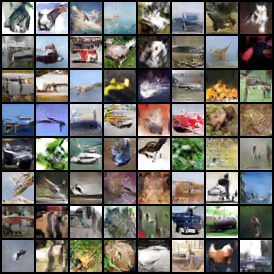
\includegraphics[width=0.6\linewidth]{figures/dcgan_baseline_grid.png}
\caption{DCGAN baseline samples}
\end{figure}


\textbf{WGAN-GP.}

WGAN-GP 在理论上改善了训练稳定性，但本实验中生成图像更模糊，目标结构较弱，定量指标也明显低于 DCGAN baseline。这说明在当前网络规模和超参数下，WGAN-GP 的稳定性优势没有转化为更好的 CIFAR-10 生成质量。


\begin{figure}[H]
\centering
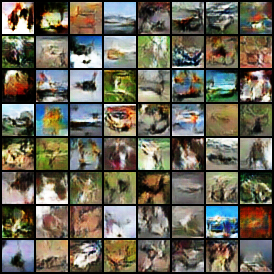
\includegraphics[width=0.6\linewidth]{figures/wgan_gp_grid.png}
\caption{WGAN-GP samples}
\end{figure}


\textbf{ResNet Conditional GAN + DiffAugment + EMA.}

ResNet 条件模型能够按照类别生成样本，因此展示图具有更明确的类别排列。不过从视觉效果和 FID/IS 来看，该模型仍存在块状纹理和类别边界不稳定的问题。其较差指标说明更复杂的条件结构需要更精细的超参数调节。


\begin{figure}[H]
\centering
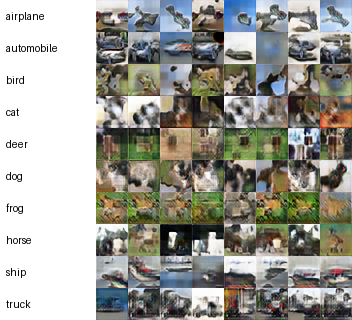
\includegraphics[width=0.6\linewidth]{figures/resnet_conditional_aug_ema_grid.png}
\caption{ResNet conditional GAN samples}
\end{figure}


\textbf{DCGAN + LSGAN + DiffAugment + EMA.}

该方法结合了最小二乘损失、可微数据增强和 EMA，但视觉质量没有超过原始 DCGAN。生成样本中仍可见较多模糊区域，说明额外训练技巧并不一定直接带来收益，需要与模型结构和优化设置配套调整。


\begin{figure}[H]
\centering
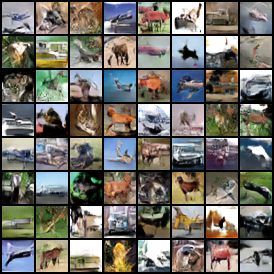
\includegraphics[width=0.6\linewidth]{figures/dcgan_lsgan_diffaugment_ema_grid.png}
\caption{DCGAN LSGAN DiffAugment EMA samples}
\end{figure}


\textbf{DCGAN + BCE + EMA, ch=64.}

在 DCGAN 上延长训练至 100 epoch 并加入 EMA 后，样本质量明显优于 50 epoch baseline。物体轮廓更稳定，背景颜色也更接近 CIFAR-10 真实分布。


\begin{figure}[H]
\centering
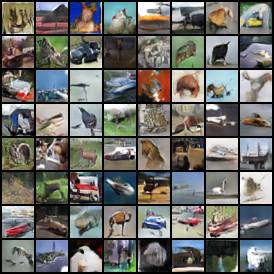
\includegraphics[width=0.6\linewidth]{figures/dcgan_bce_ema_ch64_grid.png}
\caption{DCGAN BCE EMA ch64 samples}
\end{figure}


\textbf{DCGAN + BCE + EMA, ch=96.}

将基础通道数从 64 增加到 96 后，生成样本在主体形状和颜色多样性上进一步改善。该模型曾是中间阶段的最佳结果，FID 降至 33.656，IS 提升至 5.691 ± 0.171。


\begin{figure}[H]
\centering
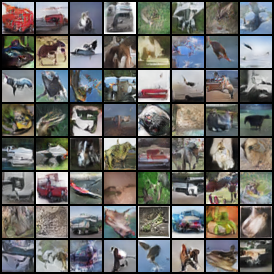
\includegraphics[width=0.6\linewidth]{figures/dcgan_bce_ema_ch96_grid.png}
\caption{DCGAN BCE EMA ch96 samples}
\end{figure}


\textbf{DCGAN + BCE + EMA, ch=128.}

继续增大到 128 通道后，样本中的车辆、船只和动物轮廓更加清楚，FID 进一步降低至 32.601。该结果说明在 ch=96 后模型仍未达到明显容量饱和。


\begin{figure}[H]
\centering
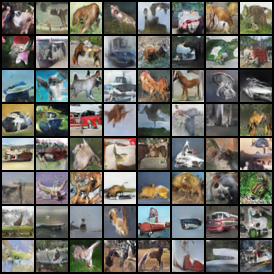
\includegraphics[width=0.6\linewidth]{figures/dcgan_bce_ema_ch128_raw_grid.png}
\caption{DCGAN BCE EMA ch128 samples}
\end{figure}


\textbf{DCGAN + BCE + EMA, ch=160.}

ch=160 raw generator 是当前最佳模型，同时取得最低 FID 和最高 IS。视觉上，该模型生成的样本具有更稳定的全局结构和更丰富的类别覆盖，但由于 CIFAR-10 分辨率仅为 32×32，细节仍然偏模糊，动物类别仍存在一定混淆。


\begin{figure}[H]
\centering
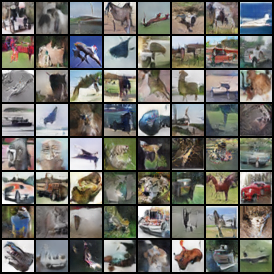
\includegraphics[width=0.6\linewidth]{figures/dcgan_bce_ema_ch160_raw_grid.png}
\caption{DCGAN BCE EMA ch160 samples}
\end{figure}


总体来看，样本对比与定量指标基本一致：WGAN-GP 和复杂条件 ResNet 模型在当前设置下没有超过 DCGAN；而沿着 DCGAN + BCE + EMA 的路线逐步增加通道数，生成质量从 ch=64、ch=96、ch=128 到 ch=160 持续提升。最终，ch=160 raw generator 在视觉效果、FID 和 IS 上均表现最好。


\subsection{类别级展示图}

最佳模型是无条件 GAN，无法直接指定类别。为了更直观展示不同语义类别的生成能力，本文从 ch=160 raw generator 采样 4000 张图像，使用预训练 Inception 特征与真实 CIFAR-10 各类别特征中心进行最近中心匹配，再为每个类别挑选最接近该类别中心的 8 张样本。该过程仅用于可视化展示，不改变模型本身。


\begin{figure}[H]
\centering
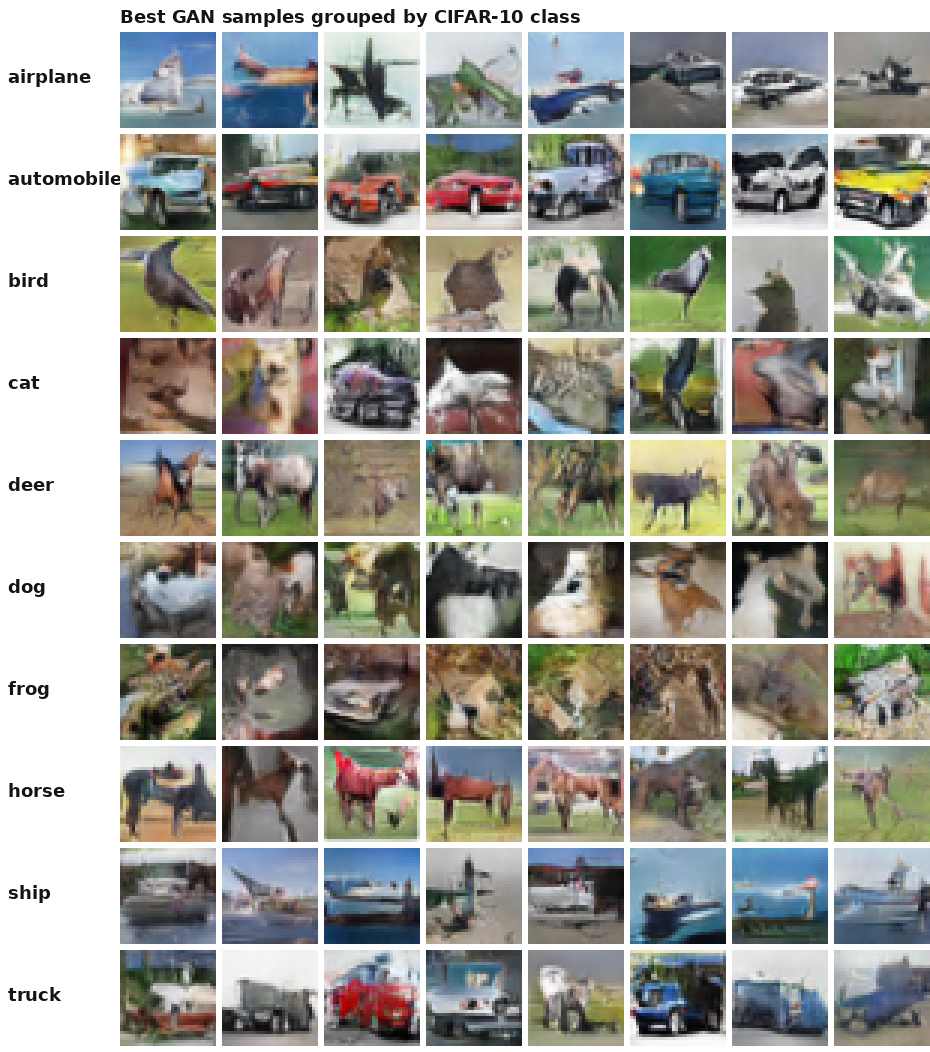
\includegraphics[width=\linewidth]{figures/dcgan_bce_ema_ch160_class_grid.png}
\caption{Class-wise generated samples}
\end{figure}


从类别展示图可以观察到，automobile、ship、truck 等刚性物体类别相对更容易形成清晰轮廓；bird、cat、dog 等动物类别更容易出现形状混淆；frog、deer 和 horse 则具有一定类别特征，但背景与主体边界仍不稳定。


\section{分析与讨论}

\subsection{为什么 WGAN-GP 没有提升结果}

WGAN-GP 理论上可以提升训练稳定性，但本实验中其 FID 明显高于 DCGAN。可能原因包括：


\begin{enumerate}
\item WGAN-GP 每轮需要更多 critic 更新，在相同 epoch 数下生成器有效更新次数和优化动态不同；
\item 当前网络容量较小，WGAN-GP 的梯度惩罚可能使 critic 学习过于保守；
\item 超参数沿用常见默认值，未针对 CIFAR-10 和本项目模型进行精细搜索；
\item FID 评价更关注最终分布匹配，而 WGAN-GP 的稳定性优势不一定直接转化为更低 FID。
\end{enumerate}


因此，本文将 WGAN-GP 作为对比实验，而非最终采用方案。


\subsection{条件 GAN 的优势与不足}

条件 GAN 的主要优势是可控生成，可以直接按类别采样，因此非常适合做类别展示。然而，本实验中条件 GAN 的 FID 和 IS 均低于最佳无条件 DCGAN。这说明条件信息虽然增强了控制能力，但也提高了优化难度。模型需要同时学习图像真实性和标签一致性，在有限训练预算下可能不如无条件模型稳定。


\subsection{ResNet 与 DiffAugment 未取得预期提升的原因}

ResNet 条件 GAN 结合 DiffAugment 和 EMA 后，视觉上能够呈现一定类别结构，但 FID/IS 结果不理想。可能原因包括：


\begin{enumerate}
\item ResNet 条件结构更复杂，对学习率、归一化方式、判别器强度和 batch size 更敏感；
\item DiffAugment 在小模型或短训练下可能改变判别器学习动态，导致生成器收到的梯度不够直接；
\item 条件模型与无条件模型使用了不同训练目标和判别器结构，最终指标并非只反映架构能力；
\item 当前实验主要面向课程项目的可运行实现，没有进行大规模超参数搜索。
\end{enumerate}


因此，复杂方法没有在本实验中胜出并不意味着其理论上无效，而是说明在当前实现和预算下，简单稳定的 DCGAN 更合适。


\subsection{EMA 与模型容量的影响}

从结果看，延长 DCGAN 训练至 100 epoch 并加入 EMA 后，FID 从 38.290 明显下降到 34.040。进一步将生成器和判别器基础通道数从 64 增加到 96 后，FID 继续下降至 33.656，IS 提升至 5.691；继续增加到 128 通道后，FID 和 IS 进一步提升；进一步增加到 160 通道后，raw generator 的 FID 降至 31.678，IS 提升至 5.872。这说明在当前训练预算下，增加 DCGAN 容量仍然能够提升分布拟合能力。


值得注意的是，在 ch=64 实验中 raw generator 的 FID 略优于 EMA，在 ch=96 实验中 EMA 同时取得更低 FID 和更高 IS，在 ch=128 实验中 raw generator 的 FID 更低、EMA generator 的 IS 更高，而在 ch=160 实验中 raw generator 同时取得更低 FID 和更高 IS。因此 EMA 的收益与训练阶段、模型容量和参数震荡程度有关，不是简单的单调提升。


\section{消融实验}

\subsection{训练轮数与 EMA}

\begin{table}[H]
\centering
\small
\begin{tabularx}{\linewidth}{lXXX}
\toprule
模型 & checkpoint & FID ↓ & IS ↑ \\
\midrule
DCGAN + BCE + EMA, ch=64 & epoch 80, EMA & 35.167 & 5.412 ± 0.173 \\
DCGAN + BCE + EMA, ch=64 & epoch 80, raw & 35.542 & 5.443 ± 0.151 \\
DCGAN + BCE + EMA, ch=64 & epoch 90, EMA & 34.468 & 5.415 ± 0.212 \\
DCGAN + BCE + EMA, ch=64 & epoch 90, raw & 35.393 & 5.492 ± 0.223 \\
DCGAN + BCE + EMA, ch=64 & epoch 100, EMA & 34.040 & 5.432 ± 0.147 \\
DCGAN + BCE + EMA, ch=64 & epoch 100, raw & 33.837 & 5.456 ± 0.183 \\
\bottomrule
\end{tabularx}
\end{table}


随着训练推进，ch=64 DCGAN 的 FID 整体下降，说明继续训练带来了有效收益。EMA 在 epoch 80 和 epoch 90 对 FID 有正向影响，但 epoch 100 时 raw generator 的 FID 略低。进一步扩大到 ch=160 后，raw generator 同时获得最低 FID 和最高 IS，因此最终报告采用 ch=160 raw generator 作为最佳模型。


\subsection{模型容量}

\begin{table}[H]
\centering
\small
\begin{tabularx}{\linewidth}{lXXX}
\toprule
模型 & 通道数 & FID ↓ & IS ↑ \\
\midrule
DCGAN + BCE + EMA & 64 & 34.040 & 5.432 ± 0.147 \\
DCGAN + BCE + EMA & 96 & 33.656 & 5.691 ± 0.171 \\
DCGAN + BCE + EMA & 128, raw generator & 32.601 & 5.834 ± 0.141 \\
DCGAN + BCE + EMA & 128, EMA generator & 32.842 & 5.851 ± 0.225 \\
DCGAN + BCE + EMA & 160, raw generator & \textbf{31.678} & \textbf{5.872 ± 0.161} \\
DCGAN + BCE + EMA & 160, EMA generator & 32.216 & 5.869 ± 0.243 \\
\bottomrule
\end{tabularx}
\end{table}


增加通道数带来更强的表示能力，使生成图像在分布匹配和类别多样性上均有所提升。


\subsection{损失函数与数据增强}

\begin{table}[H]
\centering
\small
\begin{tabularx}{\linewidth}{lXX}
\toprule
方法 & FID ↓ & IS ↑ \\
\midrule
DCGAN baseline, BCE & 38.290 & 5.346 ± 0.159 \\
DCGAN + LSGAN + DiffAugment + EMA & 41.796 & 5.163 ± 0.168 \\
DCGAN + BCE + EMA, ch=96 & 33.656 & 5.691 ± 0.171 \\
DCGAN + BCE + EMA, ch=128 raw & 32.601 & 5.834 ± 0.141 \\
DCGAN + BCE + EMA, ch=128 EMA & 32.842 & 5.851 ± 0.225 \\
DCGAN + BCE + EMA, ch=160 raw & \textbf{31.678} & \textbf{5.872 ± 0.161} \\
DCGAN + BCE + EMA, ch=160 EMA & 32.216 & 5.869 ± 0.243 \\
\bottomrule
\end{tabularx}
\end{table}


LSGAN 和 DiffAugment 的组合在本实验中未优于 BCE + EMA。这说明额外技巧需要与模型结构和超参数共同调节，直接叠加不一定带来提升。


\section{复现方式}

\subsection{训练最佳模型}

\begin{lstlisting}[language=bash]
conda run -n nern python train.py \
  --gan-type dcgan \
  --loss bce \
  --ema \
  --out-dir outputs/dcgan_bce_ema_ch160_100 \
  --epochs 100 \
  --batch-size 128 \
  --g-channels 160 \
  --d-channels 160 \
  --device cuda \
  --num-workers 2 \
  --checkpoint-every 10
\end{lstlisting}


\subsection{生成最终样本图}

\begin{lstlisting}[language=bash]
conda run -n nern python sample.py \
  --checkpoint outputs/dcgan_bce_ema_ch160_100/checkpoints/latest.pt \
  --out outputs/dcgan_bce_ema_ch160_100/final_grid_no_ema.png \
  --num-images 64 \
  --nrow 8 \
  --device cuda \
  --no-ema
\end{lstlisting}


\subsection{生成类别级展示图}

\begin{lstlisting}[language=bash]
conda run -n nern python make_class_grid.py \
  --checkpoint outputs/dcgan_bce_ema_ch160_100/checkpoints/latest.pt \
  --out outputs/dcgan_bce_ema_ch160_100/class_grid_by_nearest_centroid.png \
  --num-candidates 4000 \
  --real-per-class 1000 \
  --images-per-class 8 \
  --batch-size 128 \
  --device cuda
\end{lstlisting}


\subsection{评估 FID 和 IS}

评估 EMA generator：


\begin{lstlisting}[language=bash]
conda run -n nern python evaluate.py \
  --checkpoint outputs/dcgan_bce_ema_ch160_100/checkpoints/latest.pt \
  --out outputs/dcgan_bce_ema_ch160_100/metrics.json \
  --num-samples 5000 \
  --batch-size 64 \
  --device cuda
\end{lstlisting}


评估 raw generator：


\begin{lstlisting}[language=bash]
conda run -n nern python evaluate.py \
  --checkpoint outputs/dcgan_bce_ema_ch160_100/checkpoints/latest.pt \
  --out outputs/dcgan_bce_ema_ch160_100/metrics_no_ema.json \
  --num-samples 5000 \
  --batch-size 64 \
  --device cuda \
  --no-ema
\end{lstlisting}


\section{局限性}

尽管最佳模型在本实验范围内取得了最低 FID 和最高 IS，仍存在以下局限：


\begin{enumerate}
\item 生成图像分辨率较低，细节仍然模糊；
\item 无条件 GAN 不能直接指定类别，类别展示依赖后处理筛选；
\item 部分动物类别存在语义混淆，例如 cat、dog、deer 和 horse；
\item 实验未进行大规模超参数搜索，部分复杂方法可能没有达到最佳状态；
\item FID 和 IS 只能反映统计质量，不能完全替代人工视觉判断。
\end{enumerate}


\section{总结}

本文完成了一个面向 CIFAR-10 的 GAN 图像生成项目，实现了从训练、采样到定量评估的完整实验流程。通过比较 DCGAN、WGAN-GP、条件 GAN、ResNet 条件 GAN、DiffAugment、LSGAN 和 EMA 等方案，实验发现当前设置下最优方法是 \textbf{160 通道 DCGAN + BCE 损失}：raw generator 取得最低 FID \textbf{31.678} 和最高 IS \textbf{5.872 ± 0.161}。该方法相比基础 DCGAN 取得了明显提升，同时保持了较低实现复杂度和较好训练稳定性。


总体来看，本项目说明：在 CIFAR-10 生成任务中，复杂架构并不必然带来更优结果；合理的基线、稳定的训练策略、适当增加模型容量和严格的统一评估，往往是获得可靠实验结论的关键。


\section{参考文献}

[1] Ian Goodfellow, Jean Pouget-Abadie, Mehdi Mirza, Bing Xu, David Warde-Farley, Sherjil Ozair, Aaron Courville, and Yoshua Bengio. Generative Adversarial Nets. NeurIPS, 2014.


[2] Alec Radford, Luke Metz, and Soumith Chintala. Unsupervised Representation Learning with Deep Convolutional Generative Adversarial Networks. ICLR, 2016.


[3] Martin Arjovsky, Soumith Chintala, and Léon Bottou. Wasserstein GAN. ICML, 2017.


[4] Ishaan Gulrajani, Faruk Ahmed, Martin Arjovsky, Vincent Dumoulin, and Aaron Courville. Improved Training of Wasserstein GANs. NeurIPS, 2017.


[5] Takeru Miyato and Masanori Koyama. cGANs with Projection Discriminator. ICLR, 2018.


[6] Shengyu Zhao, Zhijian Liu, Ji Lin, Jun-Yan Zhu, and Song Han. Differentiable Augmentation for Data-Efficient GAN Training. NeurIPS, 2020.


\end{document}
